\section{Filter}

\begin{definition}[Filter]
Ein Filter $ F $ ist eine Abbildung von einem Signalraum in einen anderen, oder anders formuliert, 
ein Operator, der eine Folge $ c \in l(\Z) $ in $ Fc \in l(\Z) $ abbildet.
\end{definition}

\begin{definition}[Impulsantwort]
Die \emph{Impulsantwort} eines Filters $ F $ ist definiert als
\[
  f(k) \coloneqq (F \delta)(k), \qquad k \in \Z.
\]
\end{definition}

\begin{definition}[Transferfunktion]
Die \emph{Transferfunktion} $ \widehat{f} $ eines Filters $ F $ bezeichnet die
Fourier-Transformiertes der Impulsantwort $ f $:
\[
  \widehat{f} = \widehat{F\delta}.
\]
\end{definition}

\begin{remark}[Filtertypen]
Es gibt verschiedene Kategorien von Filtern:
\begin{description}
\item [Energieerhaltender Filter]
  In diesem Fall ist $ F : l_{2}(\Z) \rightarrow l_{2}(\Z) $ so, dass
  \[
    \norm{F}_{2} \coloneqq \sup_{\norm{c}_{2} = 1} \norm{Fc}_{2} = 1.
  \]
\item [Linearer Filter]
  Der Filter ist ein linearer Operator, d.h.\
  \[
    F(\alpha c + \beta c') = \alpha Fc + \beta Fc', \qquad \alpha, \beta \in \R, 
                                                    \quad c, c' \in l(\Z).
  \]
\item [Zeitinvarianter Filter]
  Der Operator ist \emph{stationär}, d.h.\ es ist egal, ob
  \begin{itemize}
  \item das Signal zuerst in der Zeit verschoben wird und dann Operator darauf angewendet wird,
  \item oder zuerst das Signal gefiltert und das Resultat in der Zeit verschoben wird.
  \end{itemize}
  Formal:
  \[
    F(c(\bullet + k)) = (Fc)(\bullet + k), \qquad c \in l(\Z), \quad k \in \Z.
  \]
  Oder kürzer über die Kommutativität
  \[
    F\tau_{k} = \tau_{k}F.
  \]
\item [Kausaler Filter]
  Das Ergebnis des Filters zum Zeitpunkt $ k $ hängt nur von den Eingaben in der Vergangenheit
  (also $ c(j) $ mit $ j \leq k $) ab. Der Filter kann nicht in die Zukunft sehen. Kausalität
  lässt sich auch auf"|fassen als Anforderung an die Impulsantwort des Filters: Für alle $ k > 0 $
  muss $ f(k) = (F\delta)(k) = 0 $ gelten. Einen Filter mit der Eigenschaft $ f(k) = 0 $ für alle
  $ k < 0 $ bezeichnet man übrigens als \emph{antikausal}. Einen Filter, der weder kausal noch
  antikausal ist, bezeichnet man als \emph{nicht-kausal}. Man beachte, dass nur ein nicht-kausaler
  Filter eine reellwertige Transferfunktion besitzen kann!
\end{description}
\end{remark}

\begin{remark}[Lineare und zeitinvariante Filter]\leavevmode
\begin{itemize}
\item Lineare und zeitinvariante Filter (sog.\ \emph{LTI-Filter}) können immer realisiert 
werden als \emph{Faltungen mit der Impulsantwort}. Sei also $ c \in l(\R) $ ein gegebenes diskretes 
Signal, dann gilt
\[
  Fc = c * f,
\]
wie man mit ein wenig Rechnerei nachweisen kann: Unser gegebenes Signal lässt sich auch schreiben
als
\[
  c = \sum_{k \in \Z} c(k) \ \delta(\bullet - k) = \sum_{k \in \Z} c(k) \ \tau_{-k} \ \delta
\]
und unter Verwendung der Linearität und Zeitinvarianz ergibt sich schließlich
\begin{align*}
   Fc
&= F \left( \sum_{k \in \Z} c(k) \ \tau_{-k} \ \delta \right) 
 = \sum_{k \in \Z} c(k) \ F(\tau_{-k} \ \delta)
 = \sum_{k \in \Z} c(k) \ \tau_{-k} \ F \delta
 = \sum_{k \in \Z} c(k) \ \tau_{-k} \ f \\
&= \sum_{k \in \Z} c(k) \ f(\bullet - k) = c * f.
\end{align*}
Das bedeutet, ein LTI-Filter lässt sich vollständig durch seine Impulsantwort charakterisieren.
\item Das Tolle daran ist: Dank der Faltung lassen sich LTI-Filter effizient am Rechner über eine 
Multiplikation der Transferfunktion mit der Fourier-Transformierten des Signals implementieren. 
Konkret:
\[
  Fc = \left( (Fc)^{\wedge} \right)^{\vee} = \left( (f * c)^{\wedge} \right)^{\vee}
     = \left( \widehat{f} \cdot \widehat{c} \right)^{\vee}
\]
ist sehr schnell! Denn eine Multiplikation ist wesentlich schneller und vor allem auch numerisch
stabiler durchzuführen als eine Faltung. Weiteren Zeitgewinn kann man durch Vorberechnen der
Fourier-Transformation der Impulsantwort herausschlagen. Und nicht zuletzt ist die Darstellung im
Frequenzbereich nützlich (Filterdesign funktioniert so).
\end{itemize}
\end{remark}

Von jetzt an soll die Bezeichnung \emph{digitaler Filter} immer für einen LTI-Filter stehen.

\begin{definition}[Weitere Filtertypen]
Ein digitaler Filter $ F $ heißt
\begin{enumerate}
\item \emph{FIR-Filter} (Finite Impulse Response, Filter mit endlicher Impulsantwort), wenn die
  Impulsantwort endlichen Träger hat, d.h.\ $ F\delta \in l_{00}(\Z) $.
\item \emph{IIR-Filter} (Infinite Impulse Response, Filter mit unendlicher Impulsantwort), wenn die
  Impulsantwort keinen endlichen Träger hat.
\end{enumerate}
\end{definition}

\begin{example}[FIR-Filter in der Praxis]
In der Praxis sind kausale, digitale FIR-Filter weit verbreitet. Sei $ F $ solch ein Filter mit
Impulsantwort $ f $, wobei $ \supp(f) \subseteq [0, N] $, und sei das zu verarbeitende Signal mit
$ c $ bezeichnet. Dann lässt sich der Filter angewandt auf das Signal darstellen als
\begin{align*}
  Fc &= f * c = \sum_{k \in \Z}f(k) \ c(\bullet - k) = \sum_{k = 0}^{N} f(k) \ \tau_{-k} \ c \\
     &= f(0) \ c + f(1) \ \tau_{-1} \ c + f(2) \ \tau_{-2} \ c + \ldots + f(N) \ \tau_{-N} \ c.
\end{align*}
Um $ F $ in Hardware implementieren zu können, werden also drei Bausteine benötigt: Addierer,
Multiplizierer und Verzögerer (welcher das Verschieben des Signals in der Zeit, also den
$ \tau $-Operator, modelliert).
\begin{itemize}
\item Die Verzögerer werden dazu benutzt, um nacheinander die Werte
  $ c(\bullet - 1), c(\bullet - 2), \ldots, c(\bullet - N) $ einzulesen. Für den ersten Wert $ c $ 
  braucht man keinen Verzögerer.
\item Diese Werte werden jeweils durch einen Multiplizierer mit den jeweiligen Werten
  $ f(0), f(1), \ldots, f(N) $ multipliziert.
\item Zum Schluss werden die Ergebnisse summiert nach folgendem Muster:
  \begin{itemize}
  \item $ s_{1} = f(0) \ c + f(1) \ \tau_{-1} $.
  \item $ s_{2} = s_{1} + f(2) \ \tau_{-2} $.
  \item $ s_{3} = s_{2} + f(3) \ \tau_{-3} $ usw.
  \item $ Fc = s_{N-1} + f(N) \ \tau_{-N} $.
  \end{itemize}
\end{itemize}
\TODO{Hier gehört noch das Bild hin (händisch gezeichnet aufm Tablet wär ganz gut, weil ich will
das Zeug nicht ti\emph{k}Zen)}

Die Quintessenz bei diesem Beispiel ist: Wegen der Verzögerer besitzt jeder Filter in der Praxis
eine gewisse Laufzeit.
\end{example}

\begin{remark}[Vorgehen beim Filterdesign]
Das Design eines Filters erfolgt normalerweise im Frequenzbereich. Das heißt, man stellt 
Anforderungen an die Transferfunktion (oder halt die Fourier-Transformierte des Filters), z.B.\ ob 
hohe oder tiefe Frequenzen durchgelassen werden sollen usw.
\begin{itemize}
\item Eine reelle Transferfunktion erhält man nur dann, wenn man auf Kausalität des Filters 
verzichtet. Sonst kann der Filter nicht symmetrisch sein. Die Transferfunktion eines kausalen 
Filters ist häufig komplexwertig. Dabei liefert der Realteil die Gewichtung einer Frequenz und der
entsprechende Imaginärteil legt die Phasenverschiebung fest.
\item Alle Frequenzen des Filters müssen im Intervall $ [-\pi, \pi] $ liegen. Dies ist eine 
Folgerung aus dem Abtastsatz.
\end{itemize}
\end{remark}

Es wäre jetzt natürlich schön, wenn wir jeden Filter als FIR-Filter realisieren könnten. Eine
endliche Impulsantwort ist ja eine Grundvoraussetzung dafür, dass man den Filter effizient 
implementieren kann (sonst müsste man bei der Faltung eine unendliche Summe ausrechnen). Man könnte
zwar prinzipiell jeden IIR-Filter künstlich in einen FIR-Filter umwandeln, indem man die 
Transferfunktion in einem gewissen Bereich bewusst auf $ 0 $ setzt. Dabei muss man aber aufpassen,
dass man nicht zu hart abschneidet, da der Filter an diesen Stellen sonst unangenehme Artefakte
liefern kann. Wie dem auch sei, mit solchen Problemen möchte man sich normalerweise erst gar nicht
herumschlagen. Man möchte lieber gleich einen FIR-Filter haben. Ein Problem beim Filterdesign 
besteht nun darin, dass sich aber viele Filter gar nicht als FIR-Filter realisieren lassen. Wir 
werden daher im Folgenden zunächst erkunden, welche Eigenschaften die Transferfunktion eines 
FIR-Filters erfüllen muss, und anhand dessen später ein Verfahren kennen lernen, mit dem sich ein
gewünschter Filter näherungsweise als FIR-Filter darstellen lässt.

\begin{definition}[Trigonometrisches Polynom]
Eine unendlich oft stetig differenzierbare Funktion $ f \in C^{\infty}(\T) $ der Form
\[
  f(x) = \sum_{|k| \leq n} f_{k} e^{ikx} = \sum_{|k| \leq n} f_{k} \left(e^{ix}\right)^{k}
\]
mit Koeffizienten $ f_{k} \in \C $ und Argument $ x \in \T $ bezeichnet man als trigonometrisches 
Polynom der Ordnung $ n $.
\end{definition}

\begin{remark}\leavevmode
\begin{itemize}
\item Wie bereits in der Übung bewiesen, lässt sich jedes trigonometrische Polynom der Ordnung
$ n $ auch darstellen als
\[
  f(x) = a_{0} + \sum_{k = 1}^{n} \left( a_{k}\cos^{k}(x) + b_{k}\sin^{k}(x) \right),
\]
wobei die Koeffizienten $ a_{0}, \ldots, a_{n}, b_{1}, \ldots, b_{n} \in \C $ geeignet gewählt sind.
\item Wir können direkt folgern, dass die Transferfunktion $ \widehat{f} $ zu einem 
FIR-Filter $ F $ ein trigonometrisches Polynom sein muss. Denn die Impulsantwort $ f $ hat 
endlichen Träger, sagen wir $ \supp(f) \subseteq [-N, N] $ und dann gilt ja
\[
    \widehat{f}(x)
  = \sum_{k \in \Z} f(k) e^{-ikx}
  = \sum_{k = -N}^{N} f(k) e^{-ikx} 
  = \sum_{|k| \leq N} f(k) e^{ikx},
\]
was genau der Definition eines trigonometrischen Polynoms entspricht, wenn man $ f(k) = f_{k} $
setzt.
\end{itemize}
\end{remark}

\begin{remark}[Best-Approximation einer Transferfunktion eines FIR-Filters]
Da die Transferfunktion $ \widehat{f} $ eines FIR-Filters immer ein trigonometrisches Polynom ist, 
und die trigonometrischen Polynome dicht in $ L_{2}(\T) $ liegen, ist es auch immer möglich,
$ \widehat{f} $ durch die $ n $-te Partialsumme einer Fourier-Reihe zu approximieren und durch die 
Fourier-Reihe \emph{exakt} darzustellen.
\end{remark}

\begin{example}[Approximation des Sägezahn-Filters]
Anstatt das gleiche Beispiel wie im Skript abzudrucken (idealer Tiefpassfilter), betrachten wir nun
eine Variation der Sägezahnfunktion als Transferfunktion. Diese sei definiert durch
\[
  g \colon \R \rightarrow \R, \quad g(x) = \begin{cases}
    \dfrac{\pi - x}{2}, & x \in \T \setminus \{ 0 \} \\
    0, & x = 0.
  \end{cases}
\]
Die Funktion ist offensichtlich $ 2\pi $-periodisch und \emph{kein} trigonometrisches Polynom. 
Abbildung~\ref{fig:sawtooth} zeigt den Verlauf der Funktion auf dem Intervall $ [-\pi, \pi] $.
\begin{figure}[ht]
\centering
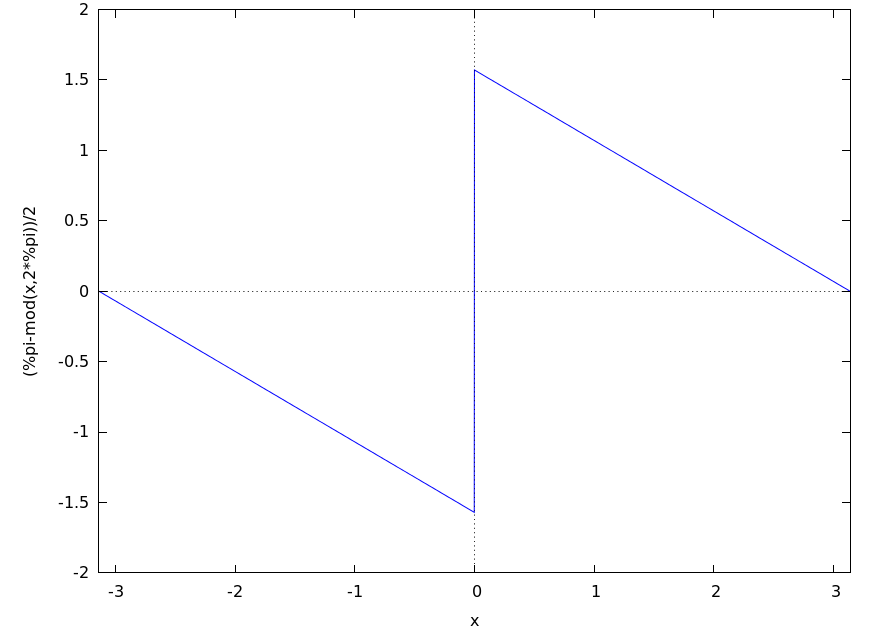
\includegraphics[width=0.5\linewidth]{Bilder/sawtooth}
\caption{Die Sägezahnfunktion $ g $ auf dem Intervall $ [-\pi, \pi] $.}
\label{fig:sawtooth}
\end{figure}
Wir wollen also ein trigonometrisches Polynom finden, welches $ g $ besonders gut annähert. Dazu
verwenden wir Fourier-Reihen. Hierfür müssen zuerst die sog.\ Fourier-Koeffizienten berechnet 
werden. Der erste Fourier-Koeffizient ist gegeben durch
\begin{align*}
   g_{0} 
&= \frac{1}{2\pi} \int_{\T} g(x) e^{- i \cdot 0 \cdot x} \dif x
 = \frac{1}{2\pi} \int_{0}^{2\pi} \frac{\pi - x}{2} \dif x
 = \frac{1}{2\pi} \left( 
     \frac{\pi}{2} \int_{0}^{2\pi} \dif x - \int_{0}^{2\pi} \frac{x}{2} \dif x
   \right) \\
&= \frac{1}{2\pi} \left( \frac{\pi}{2} \cdot 2\pi - \frac{4\pi^{2}}{4} \right)
 = \frac{1}{2\pi} \left( \pi^{2} - \pi^{2} \right)
 = 0.
\end{align*}
Für $ k \in \Z \setminus \{ 0 \} $ hingegen ergibt sich mit partieller Integration
\begin{align*}
   g_{k}
&= \frac{1}{2\pi} \int_{\T} g(x) e^{-ikx} \dif x
 = \frac{1}{2\pi} \int_{0}^{2\pi} \frac{\pi - x}{2} e^{-ikx} \dif x \\
&= \frac{1}{4\pi} \Bigg( 
      \pi \underbrace{ \int_{0}^{2\pi} e^{-ikx} \dif x }_{=0} - \int_{0}^{2\pi} xe^{-ikx} \dif x
    \Bigg)
 = -\frac{1}{4\pi} \Bigg( 
      \eval{ x\frac{e^{-ikx}}{-ik} }_{0}^{2\pi} - 
        \underbrace{ \int_{0}^{2\pi} \frac{e^{-ikx}}{-ik} \dif x }_{= 0}
    \Bigg) \\
&= \frac{1}{4\pi ik} \left( \eval{ xe^{-ikx} }_{0}^{2\pi} \right) 
 = \frac{1}{4\pi ik} \big( 2\pi \underbrace{ e^{-2\pi ik} }_{= 1} - 0 \big)
 = \frac{1}{2ik}.
\end{align*}
Damit ist die Fourier-Reihe von $ g $
\[
    \mathcal{F}g
  = \sum_{k \in \Z} g_{k} e^{ikx}
  = \sum_{k = 1}^{\infty} \frac{e^{ikx} - e^{-ikx}}{2ik}
  = \sum_{k = 1}^{\infty} \frac{\sin(kx)}{k}
\]
und deren $ n $-te Partialsumme definiert durch
\[
  \mathcal{F}_{n}g \coloneqq \sum_{k = 1}^{n} \frac{\sin(kx)}{k}.
\]
Diese $ n $-te Partialsumme verwenden wir für unseren näherungsweisen FIR-Filter. 
Abbildung~\ref{fig:sawtooth_fourier} zeigt dies exemplarisch für die Werte $ n = 5, 10, 100 $.
\begin{figure}[ht]
\centering
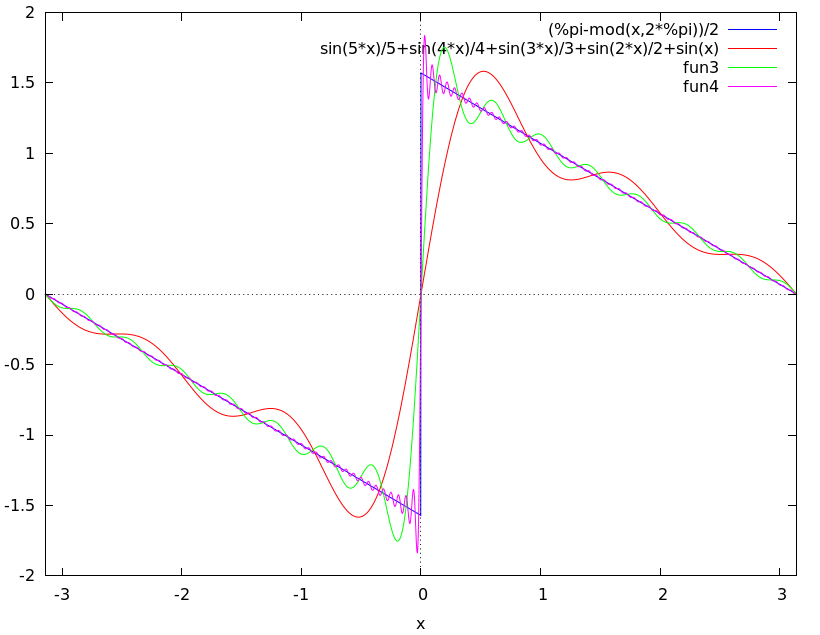
\includegraphics[width=0.5\linewidth]{Bilder/sawtooth_fourier}
\caption{Approximation von $ g $ (blau) durch die Partialsummen $ \mathcal{F}_{n}g $ für $ n = 5, 
10, 100 $ (rot, grün, lila).}
\label{fig:sawtooth_fourier}
\end{figure}
Man erkennt sehr schön, dass die Approximationsqualität für größeres $ n $ immer besser wird.
Allerdings fallen die Überschießer in der Nähe von $ x = 0 $ (hier macht die Funktion zwei Sprünge) 
unangenehm auf. Diese werden mit zunehmendem $ n $ zwar immer schmaler, aber eben nicht kleiner.
Diese Beobachtung bezeichnet man auch als \emph{Gibbs-Phänomen}. Dies macht Fourier-Reihen zur 
Approximation von Bandpassfiltern nicht immer zur besten Wahl.

Man kann versuchen, die problematischen Überschwinger und Oszillationen zu glätten. Dafür definieren
wir uns die \emph{Fej\'{e}r'schen Mittel}:
\[
  \mathcal{G}_{n} \coloneqq \frac{1}{n + 1} \sum_{k = 0}^{n} \mathcal{F}_{k}, \quad n \in \N.
\]
Anstatt nur eine Partialsumme $ \mathcal{F}_{n} $ betrachten wir also das arithmetische Mittel 
aller Partialsummen $ \mathcal{F}_{0}, \mathcal{F}_{1}, \ldots, \mathcal{F}_{n} $. Die 
Fej\'{e}r'schen Mittel sind für Werte von $ n = 5, 10, 100 $ in Abbildung~\ref{fig:sawtooth_fejer}
dargestellt.
\begin{figure}[ht]
\centering
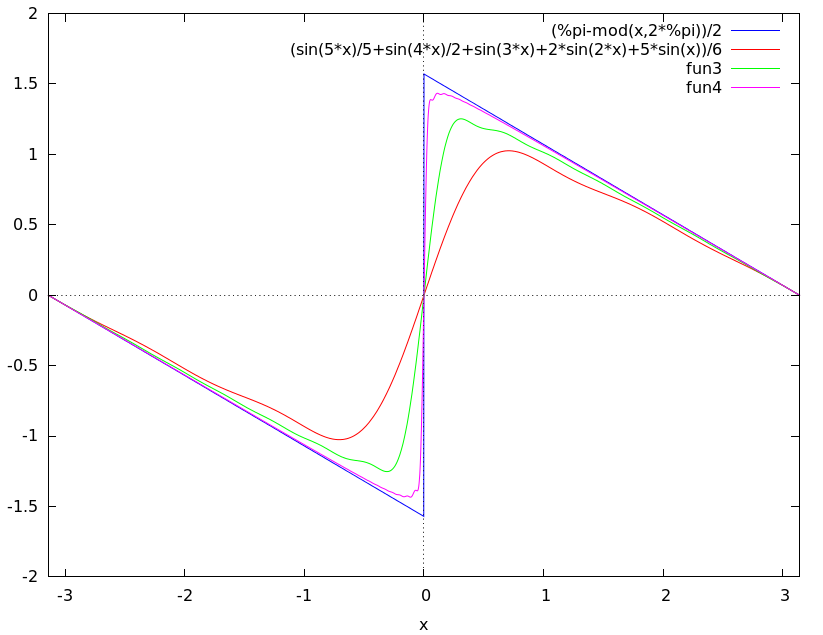
\includegraphics[width=0.5\linewidth]{Bilder/sawtooth_fejer}
\caption{Approximation von $ g $ (blau) durch die Fej\'{e}r'schen Mittel $ \mathcal{G}_{n}g $ für 
$ n = 5, 10, 100 $ (rot, grün, lila).}
\label{fig:sawtooth_fejer}
\end{figure}
Man sieht recht schön, dass diese zwar eine größere Abweichung von $ g $ aufweisen als die
$ n $-ten Partialsummen der Fourier-Reihe von $ g $. Dafür vermeiden sie aber das Gibbs-Phänomen.
\end{example}